\section{Introduction to ABC-SysBio}







\section{Methods}
%\subsection{\acrshort{abc} for parameter estimation}



\subsection{\acrshort{abc} for model selection}
Given the range of parameter values shown to give rise to bistability during the parameter scan shown above, a sample of those were used as priors for ABC SMC parameter inference. The initial conditions were set to gA = 1.0, gB = 1.0 and A2 = 10. Thus the system began at the off state. An inducer is added at t=20 and another one at t=70. The model is shown below and the distance function used is shown in the Appendix. The results are shown in Figure~\ref{XXX}. The target behaviour to which the model was compared to is shown in Figure~\ref{fig:behaviour}.

The standard toggle switch model was shown to successfully behave like a switch within the parameter range used here. As a next step it will be examined whether the addition of feedback loops can make the switching more robust to parameter changes. It is predicted that the addition of feedback loops will increase the robustness of the switch and thus be selected over the standard toggle switch.

Model selection can arise from the ABC SMC methodology naturally, by adding the model as an unknown parameter to the selection process. A model and its parameter values, \texttheta, are sampled from the prior distribution. Using these parameter values the sampled model is simulated and the distance between the resulting time course and the target time course measured. The algorithm then proceeds as described previously, by sampling each time models and parameters from their priors. When the last \textepsilon{} is reached, the algorithm will have concluded to a posterior distribution of parameters for each model, a subset of the prior distribution that can give the best rise to the data. The model that performs over a greater posterior parameter range is selected as the most robust~\autocite{Toni:2009tr}.  
    

%\begin{figure}[h!]
%    \centering
%    \hspace*{-1cm}
%    \includegraphics[scale=0.7]{Images/abc_model_s}
%    \caption{ABC algorithm.  }
%    \label{fig:abc_explain}
%\end{figure}

In order to select for the more robust toggle switch, the standard toggle switch will be compared to switches with positive or negative auto-regulation in one or both nodes as shown in Figure~\ref{fig:toggle_switch_designs}. There are two inducers, one turning the switch on by repressing A and one turning the switch off by repressing B. %The stimulus could be a transcription factor occupying the promoter region %or red and far-red light ~\cite{Muller:2013ew}. 
    The reactions of the standard toggle switch are shown in Appendix (XXX). Given the models shown above and the parameter priors used for the standard toggle switch parameter inference, ABC SMC model selection will be carried out. Using the ABC SMC model selection, the most robust model can be selected. The most robust model is the model that can produce the same behaviour over a greater range of parameters. 

\begin{figure*}[htbp]
	\begin{center}
\includegraphics[scale=0.5]{chapterABCSysBio/images/model_selection.png}
\caption[LoF caption]{\label{fig:abc_model_sel}: Model selection}
\end{center}
\end{figure*}
\clearpage

\subsection{Particle sampling}
\label{sec:part_samp}
For the first population, particles are sampled from the priors. Random samples are taken from the distribution specified by the user for each parameter. 

For subsequent populations particles are sampled from the previous population. The weight of each particle in the previous population dictates the probability of it being sampled. The number of samples to be drawn is specified by the user in the input file.  

\subsection{Perturbation}
\label{sec:pertub}
Each sampled particle is perturbed by a kernel defined by the distribution of the previous population, as developed by~\textcite{Toni:2009tr}. 

\begin{align}
K_p(\theta|\theta* ) =& \theta* + U(+s_p, -s_p)\text{, where:} \\
s_p =& \frac{1}{2} \big (max(\theta_{p-1}) - min(\theta_{p-1}) \big )
\end{align}

If the \texttheta* falls out of the limits of the priors then the perturbation is rejected and repeated until an acceptable \texttheta* is obtained. This method is successful in perturbing the particles by a small amount in order to explore the parameter space, but can be slow to complete. 

\subsection{Particle simulation}
\label{sec:sim}
Each particle is simulated using cuda-sim~\autocite{Zhou:2011hp}. The model is provided by the user in SBML format and is converted into CUDA\textsuperscript{\textregistered} code by cuda-sim. The model in CUDA\textsuperscript{\textregistered} code format can then be run on NVIDIA\textsuperscript{\textregistered}. CUDA\textsuperscript{\textregistered}. \acrshort{gpu}s. This allows the user to take advantage of the speed of parallelised simulations without any CUDA\textsuperscript{\textregistered} knowledge. 

\subsection{Distance function}


\begin{figure*}[htbp]
	\begin{center}
\includegraphics[scale=0.7]{chapterABCSysBio/images/behaviour.png}
\caption[LoF caption]{\label{fig:abc_behav}: Selected behaviour}
\end{center}
\end{figure*}


\begin{align*}
	d_1 &= \sum_{i=0}^{20} (s_i-t_1)^2 \\
	d_2 &= \sum_{i=21}^{70} (s_i-t_2)^2 \\
	d_3 &=  \sum_{i=71}^{100} (s_i-t_3)^2, \\
\end{align*}
where $i$ represents the timepoints, $s_i$ the simulation result at  each timepoint and $t1 = 0$, $t2 = 20$, $t3 = 0$ represent each target behaviour.

\subsection{Weight calculation}
\label{sec:weight}
For the first population the weights are all given a value of 1, and then normalised over the number of particles. For subsequent populations the weights of the particles are calculated by considering the weights of the previous population~\autocite{Toni:2009tr}. 

\begin{align}
w_{t}^{(i)} = \frac{P(\theta_{t}^{(i)})}{\sum_{j=1}^N w_{t-1}^{(j)} K_{t}(\theta_{t-1}^{(j)}, \theta_{t}^{(i)})} \text{ for n $\textgreater$  0}
\end{align}
	
The weights are then normalised over the total number of particles. 
    
%\section{Models of the genetic toggle switch}
%\section{Results}
\section{Genetic toggle switch model selection}
    
$$
\begin{array}{cccc}
      \textrm{gA}\stackrel{\textrm{ge}}{\longrightarrow}\textrm{gA} + \textrm{A} \\
      \textrm{gB}\stackrel{\textrm{ge}}{\longrightarrow}\textrm{gB} + \textrm{B} \\
      \textrm{A} + \textrm{A} \stackrel{\textrm{dim}}{\longrightarrow}\textrm{A2} \\
      \textrm{A2} \stackrel{\textrm{dim r}}{\longrightarrow}\textrm{A} + \textrm{A} \\
      \textrm{B} + \textrm{B} \stackrel{\textrm{dim}}{\longrightarrow} \textrm{B2} \\
      \textrm{B2} \stackrel{\textrm{dim r}}{\longrightarrow}\textrm{B} + \textrm{B} \\
      \textrm{gA} + \textrm{B2} \stackrel{\textrm{rep}}{\longrightarrow}\textrm{B2gA} \\
      \textrm{B2gA} \stackrel{\textrm{rep r}}{\longrightarrow}\textrm{B} + \textrm{gA} \\
      \textrm{gB} + \textrm{A2} \stackrel{\textrm{rep}}{\longrightarrow}\textrm{A2gB} \\
      \textrm{A2gB} \stackrel{\textrm{rep r}}{\longrightarrow}\textrm{A2} + \textrm{gB} \\
      \textrm{A} \stackrel{\textrm{deg}}{\longrightarrow}\textrm{\O}\\
      \textrm{B} \stackrel{\textrm{deg}}{\longrightarrow}\textrm{\O}\\
      \textrm{S} + \textrm{A2} \stackrel{\textrm{rep dim}}{\longrightarrow}\textrm{SA2}\\
      \textrm{SA2} \stackrel{\textrm{rep dim r}}{\longrightarrow}\textrm{S} + \textrm{A2}\\
      \textrm{R} + \textrm{B2} \stackrel{\textrm{rep dim}}{\longrightarrow}\textrm{RB2}\\
      \textrm{RB2} \stackrel{\textrm{rep dim r}}{\longrightarrow}\textrm{R} + \textrm{B2}\\
      \textrm{R} \stackrel{\textrm{deg}}{\longrightarrow} \textrm{\O}\\
      \textrm{S} \stackrel{\textrm{deg}}{\longrightarrow}\textrm{\O}\\
\end{array}
$$

\paragraph{}

The toggle switches with positive or negative autoregulation have the same set of equations with the addition of the ones shown below. Toggle switches with autoregulation on both transcription factors have both relevant sets:

\paragraph{Positive autoregulation on A:}

$$
\begin{array}{cccc} 
    \textrm{A2} + \textrm{gA} \stackrel{\textrm{aut 1}}{\longrightarrow} \textrm{A2gA} \\
    \textrm{A2gA} \stackrel{\textrm{aut 2}}{\longrightarrow} \textrm{A} + \textrm{A2gA}\\
    \textrm{A2gA} \stackrel{\textrm{aut 3}}{\longrightarrow} \textrm{A2}+ \textrm{gA}  \\
\end{array}
$$
\paragraph{Positive autoregulation on B:}

$$
\begin{array}{cccc} 
    \textrm{B2} + \textrm{gB} \stackrel{\textrm{aut 1}}{\longrightarrow} \textrm{B2gB} \\
    \textrm{B2gB} \stackrel{\textrm{aut 2}}{\longrightarrow} \textrm{B} + \textrm{B2gB}\\
    \textrm{B2gB} \stackrel{\textrm{aut 3}}{\longrightarrow} \textrm{B2}+ \textrm{gB}  \\
\end{array}
$$

\paragraph{Negative autoregulation on A:}

$$
\begin{array}{cccc} 
    \textrm{A2} + \textrm{gA} \stackrel{\textrm{aut 1}}{\longrightarrow} \textrm{A2gA} \\
    \textrm{A2gA} \stackrel{\textrm{aut 2}}{\longrightarrow} \textrm{A2}+ \textrm{gA}  \\
\end{array}
$$
\paragraph{Negative autoregulation on B:}
$$
\begin{array}{cccc} 
    \textrm{B2} + \textrm{gB} \stackrel{\textrm{aut 1}}{\longrightarrow} \textrm{B2gB} \\
    \textrm{B2gB} \stackrel{\textrm{aut 2}}{\longrightarrow} \textrm{B2}+ \textrm{gB}  \\
\end{array}
$$


\begin{figure*}[htbp]
	\begin{center}
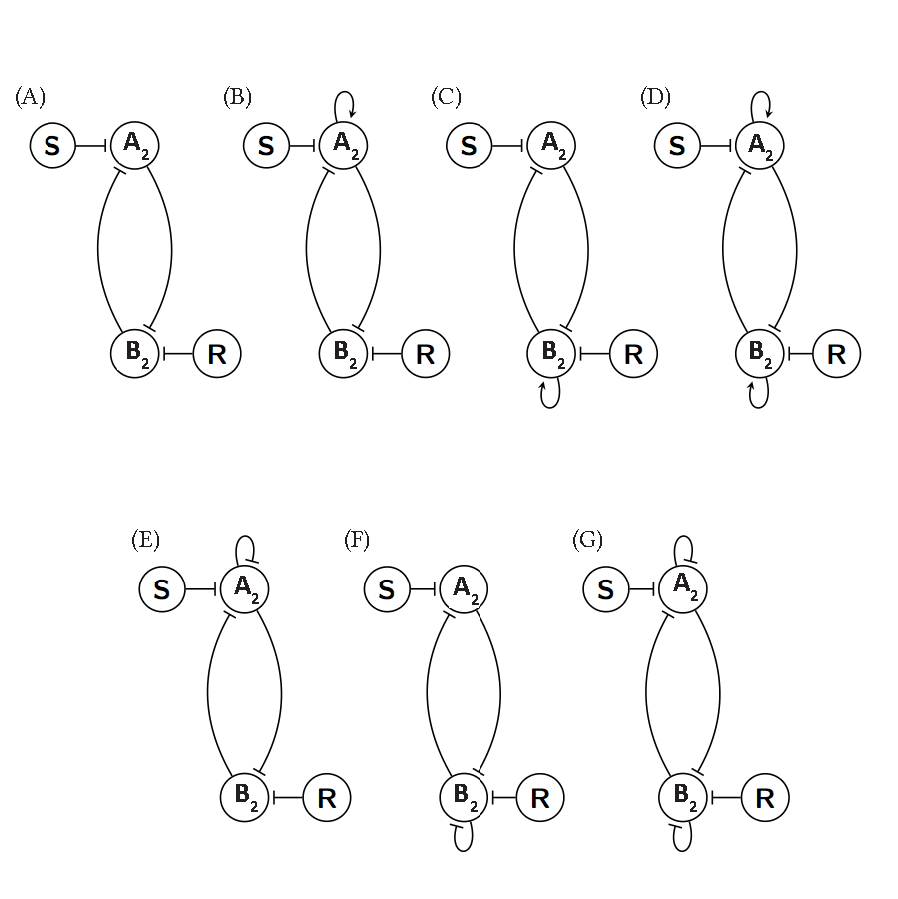
\includegraphics[scale=0.7]{chapterABCSysBio/images/toggle_switch_designs.png}
\caption[LoF caption]{\label{fig:toggle_switch_designs}: Toggle switch designs used for model selection}
\end{center}
\end{figure*}
\clearpage
\section{Discussion}
\section{Summary}

In this chapter I...


